\documentclass[conference]{csce}

\usepackage[hmargin=.75in,vmargin=1in]{geometry}
\usepackage[american]{babel}
\usepackage[T1]{fontenc}
\usepackage{times}
\usepackage{caption}
\usepackage{amsmath}
\usepackage{graphicx}
\usepackage{tikz}
\usepackage{moreverb}
\usepackage{url}
\usepackage{subcaption}
\usepackage{verbatim}
% double spacing
\usepackage{setspace}

%%% Class name, option, and packages above are mandatory for generating an appropriate format 
%%% suitable for the CSCE style. Therefore, do not make any changes unless you know 
%%% what you are doing.
%%% However, if you need to use the subfig package, you must call it BEFORE the caption package.
%%% (NOTE: the subfig package probably will work but has not been tested.)

%%% The csce.cls is derived (in a quite dirty and quick manner) from the IEEEtrans.cls.
%%% At least the following packages are incompatible with the csce.cls:
%%% <DO NOT USE THEM> setspace, titlesec, amsthm
%%% There may be more, so if you use a package that produces a lot of errors or weird results, 
%%% be advised to avoid that package.

%%% Below packages are recommended to use for better results and compatible with the csce.cls
\usepackage{textcomp}
\usepackage{epsfig,graphicx}
\usepackage{xcolor}
\usepackage{amsfonts,amsmath,amssymb}
\usepackage{fixltx2e} % Fixing numbering problem when using figure/table* 
\usepackage{booktabs}

%%% Below packages are probably useful for some table-formatting purposes. Compatibility is not yet
%%% tested but probably fine.
%\usepackage{tabularx}
%\usepackage{tabulary}

%%% Using the hyperref package is not really necessary for conference papers, but if your paper includes
%%% a lot of URLs, and you wish them to be line-breakable, it might be useful.  When you need to use the
%%% hyperref package, make sure you set <colorlinks option> = true and all link colors black as shown in
%%% the sample below (the sample calls the ifpdf package, too).
%\usepackage{ifpdf} 
%\ifpdf
%\usepackage[pdftex,naturalnames,breaklinks=true,colorlinks=true,linkcolor=black,citecolor=black,filecolor=black,menucolor=black,urlcolor=black]{hyperref}
%\else
%\usepackage[dvips,naturalnames,breaklinks=true]{hyperref}
%\fi

\columnsep 6mm  %%% DO NOT CHANGE THIS


\title{\bf Applying Genetic Algorithms to Generating Paintings}           %%%% Replace with your title.

%%%% Replace the author and institution/affiliation names. 
%%%% Make sure the author names are boldface.
\author{
{\bfseries Alexander Hansen$^1$ and  Mark. C. Lewis$^1$}\\
$^1$Department of Computer Science, Trinity University, San Antonio, Texas, USA\\
}

\begin{document}


\maketitle                        %%%% To set Title and Author names.


\begin{abstract}%%%% Replace with your abstract.
Please consider these Instructions as guidelines for preparation of 
Final Camera-Ready papers. The Camera-Ready Papers would be acceptable as 
long as it is formatted reasonably close to the format being suggested here. 
Note that these instructions are reasonably comparable to the standard IEEE 
typesetting format. Type the abstract (100 words minimum and 150 words maximum) 
using Italic font with point size 10. The abstract is an essential part of the 
paper. Use short, direct, and complete sentences. It should be brief and as concise as possible.
\end{abstract}


\vspace{1em}
\noindent\textbf{Keywords:}
 {\small  A maximum of 6 keywords} %%%% Replace with your keywords

%%%%%%%%%%%%%%%%%%%%%%%%%%%%%%%%%%%%%%%%%%%%%%%%%%%%%%%%%%%%
% problem

%TODO: it would be fun to create an image based on one photo and do the fitness with respect to another photo

%TODO: appendix of photos run through the painter
%TODO: Insert a narrative of finding the balance of computational work and good fitness/visual results

\chapter{Applying Genetic Algorithms to Generating Paintings Based on Images}
\section{Introduction}

This project explores the application of genetic algorithms to generating paintings based on photos. We find various combinations of parameters for our genetic algorithm that strike a balance between computational work and visually pleasing and accurate results. 

\subsection{Background Information}
The subject of generating paintings based on algorithmic operations applied to computers has been studied before in great depth.\cite{synergistic}\cite{monet}\cite{organicpainting} These approaches are highly effective and expressive, but some can be stylistically limited due to their deterministic nature of analysis. In the case of both \cite{synergistic} and \cite{monet}, they analyze features from the original image, such as color or edge location, and abstract them into something that can become a stroke or collection of strokes and represent them in a table. The painting algorithm draws from this table to ensure the feature is represented in the final rendered painting. This is the approach of most painting algorithms that are based on an original image. Those other algorithms which paint images based on no original reference image, such as \cite{organicpainting}, are a different problem than this project, so they will be referred to sparingly. 

As it is hard to say in art whether one approach is better or worse, this project seeks not necessarily to improve upon the previous work but to provide another entirely different tool for generating paintings based on a reference image. We utilize machine learning, specifically a genetic algorithm, to create a large amount of paintings and then evolve them into one, particularly accurate, painting. This accuracy is determined by a fitness function which is discussed later. 

The concept of a genetic algorithm was originally proposed by A.S. Fraser with the intent of being able to computerize and simulate evolution.\cite{fraser1957simulation} Originally, it was much more focused on the mutation and mating aspects of it, and less on the fitness definition and iteration. In applying genetic algorithms to art, however, a creative use of a fitness function and a mutation function are required. 

Much work has been done on genetic algorithms, and they seem to contain an inherent quality that makes them good at optimization problems. This can be seen in the amount of publications across many diverse fields using genetic algorithms to optimize their problems. Some examples are molecular geometry calculations,\cite{molecular} electromagnetic design tools,\cite{electro} course scheduling.\cite{courses} There is much more work out there exemplifying this optimization characteristic. \cite{genetic1}\cite{genetic2}\cite{genetic3}\cite{genetic4}\cite{genetic5}

Genetic algorithms are often applied to optimization problems in this way because they are able to find optimal solutions without necessarily knowing why they are optimal. In problems where there are features that can be evaluated and weighted based on how good or bad they are with respect to the final product, genetic algorithms are able to find optimal arrangements of these features. We apply this to paintings, as every stroke can be viewed as a feature and evaluated in this way. Some work has been done on applying genetic algorithms to art and in very interesting ways. Karl Sims has published a paper and created an art exhibit using one.\cite{sims} He, too, struggles with large parameter spaces in his work and discusses some ways around them, but his process is not based on a reference image as ours is, so we cannot take advantage of these approaches. %TODO study these

Sims also has an exhibit where there are sixteen different paintings, and visitors to the exhibit can select the most visually appealing ones. Their features are then mixed to create the next generation of paintings. This is a good demonstration of the idea behind genetic algorithms.

Other work on using genetic algorithms with art include Roger Johansson's implementation in Javascript of a genetic algorithm to approximate the best arrangement of fifty polygons to replicate the Mona Lisa with great success.\cite{monalisa} This project can be viewed online. \footnote{It can be viewed here: https://chriscummins.cc/s/genetics/}


\section{Implementation}

\subsection{Applying a Genetic Algorithm to Painting}
There are three core parts to this project: the generation function, the genetic algorithm, and the rendering. Paintings are a struct represented by a collection of strokes, which is a struct with a start point, an end point, a width, and a color. 

The genetic algorithm itself has five parts: the selector function, which selects which of the population to mate; the fitness function, which defines the fitness of a painting; the crossover function, which defines how two paintings interact to create a child; the mutation function, which randomly mutates a painting; and the simulator, which iterates the genetic algorithm according to some given properties and kills off stochastically.

The structure of the program, from a high level, is as follows:
\begin{enumerate}
    \item The generator function generates $n$ initial random paintings.
    \item The selector function selects $m$ of the initial random paintings to mate and produce child paintings.
    \item The crossover function takes two selected paintings and combines their strokes, half from one and half from the other, to create a child painting. It repeats this process until all of the selected paintings have been mated.
    \item Another selector function selects $o$ random members of the population.
    \item The mutation function mutates these $o$ members.
    \item The simulator then stochastically kills off $m$ paintings from the population.
    \item Go back to step 2 and repeat until a predetermined number of iterations has been met.
    \item Render the most fit, according to the fitness function, of the population and output it as the final result.
\end{enumerate}

\subsection{The Fitness Function}
This paper will frequently refer to the ``fitness'' of a painting. This is a value determined by the fitness function. It is therefore crucial to explain first, as the rest of the discourse in this paper relies on this concept. The fitness function gives us an integer value for how ``good'' a painting is with respect to the original photo. This allows the various parts of the simulator to address photos by how fit they are and make decisions accordingly. It also provides us with a quantitative metric with which to compare the effectiveness of various approaches and tweaks to our program.

In our problem, we want to take an image and turn it into a painting. One of the most basic concepts of how accurate a painting is to a given reference photo is how far off the color is of every pixel. For example, given the RGB values of original photo pixel located at $(1, 1)$ as $(255, 254, 255)$ and the corresponding painting pixel located at $(1, 1)$ as $(255, 255, 255)$, we can see that the $G$ value is one pixel off from the original. This gives it an ``unfitness'' of $1$. We can take the inverse of this to get the fitness. The inverse is the maximum possible difference ($255 + 255 + 255 = 765$) minus the actual difference ($1$), so $765 - 1$. Therefore, this particular pixel in the painting has a fitness of $764$. The fitness value of a painting is the sum of the fitness of every rendered pixel in comparison to the original photo.

Note that the fitness function does not rely on mutating any data, only referencing the two images. This means that it is easily implemented in parallel, a feature that is important in executing genetic algorithms in a timely manner. The actual code for this function can be seen in the appendix as Figure \ref{fitnesscode}. 



\subsection{The Rendering Function}

Rendering a painting is as minimalist and intuitive. From the start point to the end point of every stroke, a line is drawn with the stroke's color. This line has the width of the stroke's width. There is no actual paint simulation or anything particularly advanced happening here. This is because the discoloration of paint or lighting could interfere with the fitness function's ability to accurately compare the color of a stroke to the original photo. 

The rendering function is important to this project because it is used in the calculation of the fitness and therefore the assessment of the genetic algorithm's progress and quantitative results.


Figure \ref{fig:refvsfinal} shows an example of a rendered painting with it's original image next to it. 
\begin{figure}
\begin{subfigure}[t]{.5\linewidth}
      \centering
      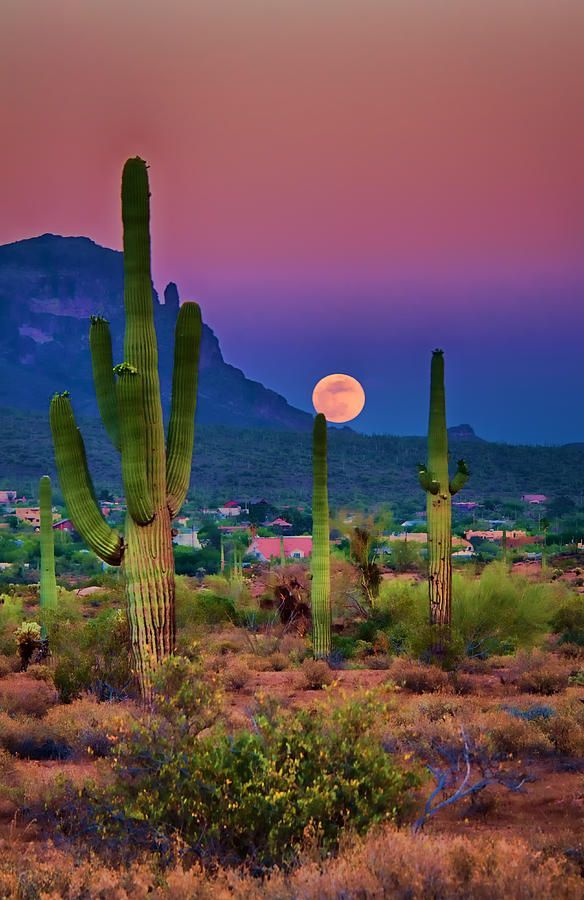
\includegraphics[width=0.4\linewidth]{reference.jpg}
  \end{subfigure}%
  \begin{subfigure}[t]{.5\linewidth}
      \centering
      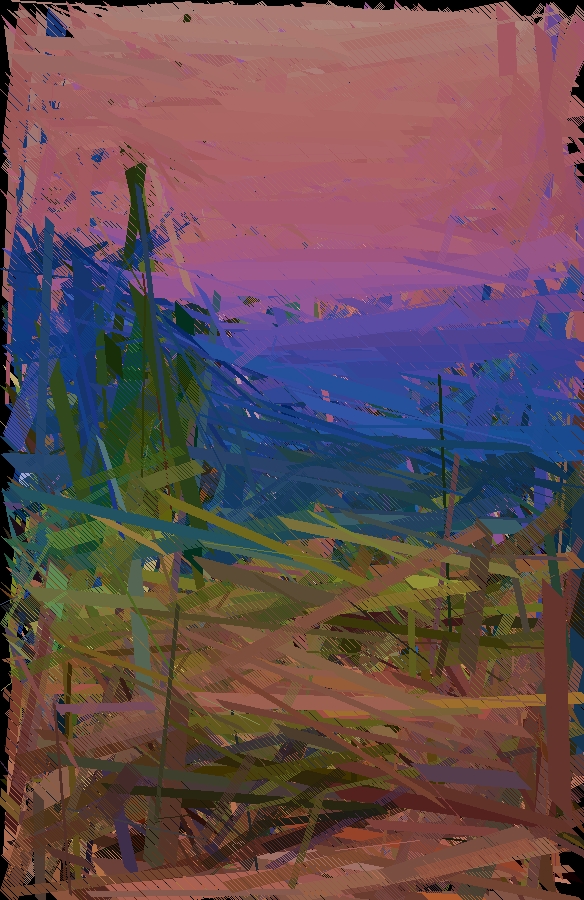
\includegraphics[width=0.4\linewidth]{informed.png}
  \end{subfigure}
  \caption{A rendered painting with its original reference image to the left of it}
    \label{fig:refvsfinal}
\end{figure}


\subsection{The Generator Function}
The generator function is the function that generates random paintings for the initial population of the genetic algorithm. Originally, it was truly random, generating completely random strokes with completely random parameters and combining them into a painting. This was not good enough. The parameter space of the problem is too large. Strokes have color, length, position, width, etc., and starting with truly random strokes puts us so far away from an optimal solution that it takes the genetic algorithm far too many iterations to get a desirable result. We instead created an ``informed'' random generator. In this improved generator, most aspects are still kept random but certain things are set to be more accurate by taking some features from the reference image. We limited the minimum and maximum length of strokes to be set by an argument passed in by the user, which minimizes the parameter space greatly. We also set the color of every stroke to be the color of the original image at its start position, and thus further shrank the parameter space. This proved to greatly increase starting fitness. Note that the fitness increase did not sacrifice the effectiveness of the genetic algorithm. The final fitness is a function of the starting fitness, as seen below. In Figure \ref{fig:informedvsrandom}, we introduce the ``fitness graph'' which is a graph of the maximum fitness at every iteration through an execution of our genetic algorithm, to show the difference in both fitness and final image when an informed random generation function is used versus a purely random one. 


\begin{figure}
\centering
  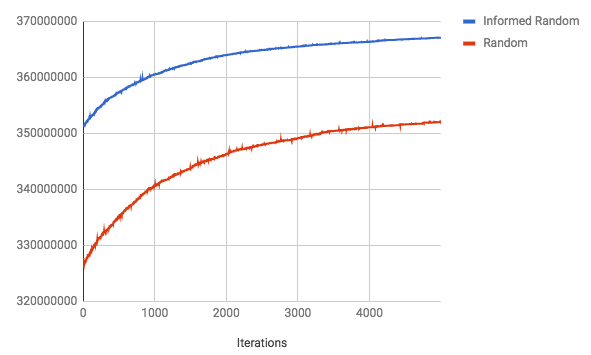
\includegraphics[width=\linewidth]{InformedvsRandom.png}
  \centering
  \begin{subfigure}[t]{.5\linewidth}
      \centering
      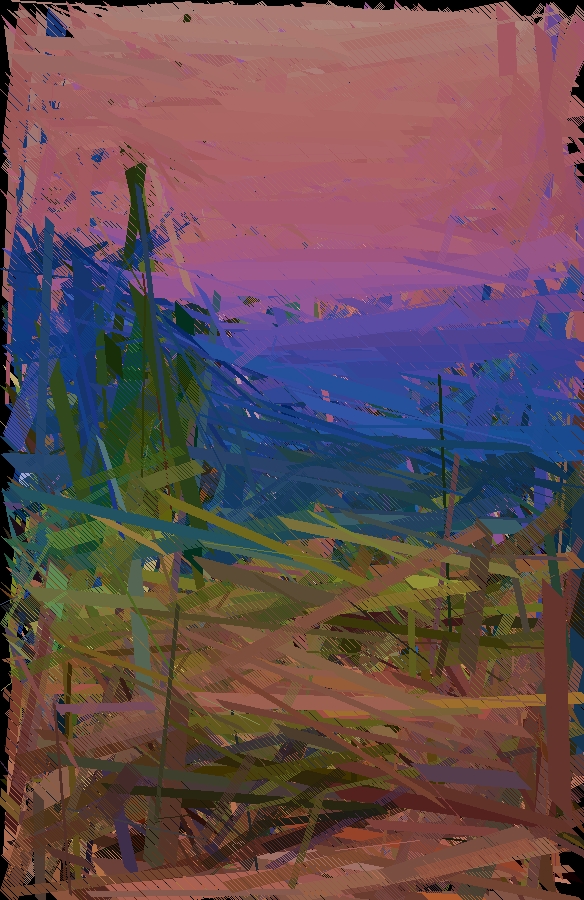
\includegraphics[width=0.4\linewidth]{informed.png}
      \caption{Informed random final result.}
  \end{subfigure}%
  \begin{subfigure}[t]{.5\linewidth}
      \centering
      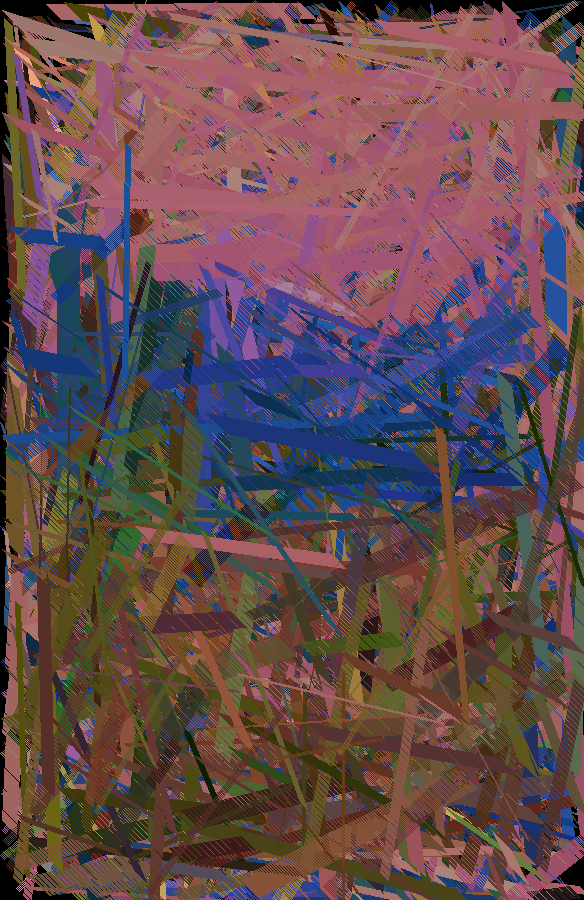
\includegraphics[width=0.4\linewidth]{random.png}
      \caption{Random final result.}
  \end{subfigure}
    \caption[Informed random generation compared with fully random generation]{The maximum fitness of every iteration's population using the informed random generation approach versus the non-informed approach, and their respective final results from the genetic algorithm after 5000 iterations.}
  \label{fig:informedvsrandom}
\end{figure}


\subsection{The Selector Function}
The selector function's job is to select which parents will mate to produce the children for the next iteration.

There are different kinds of selectors that are used in genetic algorithms. There is stochastic, which is random and is effectively useless for this application; there is tournament selection, which chooses $x$ members of the population at a time to participate in a tournament and picks the top $2$ most fit participants from that tournament (multiple tournaments can be run per iteration); fitness maximal selection, which selects the absolute most fit members to mate; and some other more obscure types.


The amount parents being selected to "mate" each iteration is an input to these selector functions. So, the maximize selector picks the top $x$ to mate, producing $\frac{x}{2}$ children. This is a parameter that we fixed to $\frac{n}{3}$, where $n$ is the total population size, producing $\frac{n}{6}$ of the population size children every iteration, and killing off $\frac{n}{6}$ as well. We tested a few other values, but ultimately fixed it to $\frac{n}{3}$ as it seemed optimal. This is discussed more in the results section. Fixing this value, although semi-arbitrary, provided consistency as we tested the other elements of the genetic algorithm's parameter space, which was already far too large. The maximize selector was our primary choice as it picks the most fit paintings and then uses them to create children. This can cause a phenomenon of a local maxima, but it still resulted in the highest fitness. That is, the local maxima level is higher in the maximize function than the highest fitness able to be achieved by other selectors in the same amount of time. This will be discussed more in the results section.

The tournament selector was the other selector we experimented with. It takes two parameters: the number of tournaments and the number of participants in the tournament. We fixed these values, again somewhat arbitrarily, to $\frac{n}{6}$ tournaments of size $\frac{n}{10}$. For a population size of $1000$, this would be $166$ tournaments of size $10$. This results in $1660$ fitness calculations per iteration, which is more than the maximize selector, but is often more efficient as it will select the same population member multiple times and access the cached fitness value. The scaling of the tournament selector is independent of the fitness increase, meaning it is not just a slower maximize selector.\cite{selectors} This means it could be resistant to the local maxima that the maximize selector can sometimes experience.


\subsection{The Crossover Function}
After a subset of the population has been selected to become ``parents'', they are passed into a crossover function. In the original definition of a genetic algorithm, this was a function that took the two parents' binary string representations and split them, combining part from one parent and part from the other.\cite{fraser1957simulation}

We approximate this process; instead of using a binary representation, we take half of the strokes from one painting and half of the strokes from the other, combining them. To maximize the increase in fitness, we compare the two potential combinations (parent one's first half, and then parent two's, or vice versa), and pick the best combination. This worked, but also made us more susceptible to local maxima, also known as Hamming walls. This will be discussed later in the results section. Because of this, this feature was removed. Some other versions of the crossover function exist, such as not taking exactly half from each painting and instead taking a random percentage from each that totals one hundred percent, but no major improvement in performance was shown using this method.
This new set of child paintings are then added into the total population.

\subsection{The Mutation Function}
After the child paintings are added to the population, a stochastic selector function selects a predetermined amount of paintings to mutate. We decided that we would pick a random parameter of a stroke and modify it by a predetermined ``mutation strength''. The code of our original implementation of the mutation function is available as Figure \ref{fig:origmutation} in the appendix. You will notice that in the end, this function, like the original crossover function, also makes a comparison to ensure a better fitness. The painting compares itself to its pre-mutated state and picks the more fit painting to return. This also made us more susceptible to Hamming walls, and was removed. The mutation strength is better as a relatively large value to help avoid Hamming walls. 

After the mutation occurs, a number of paintings equivalent to the amount of child paintings that were just added are stochastically selected to be ``killed'', or removed from the population.

\section{Results}
\subsection{Maximizing Fitness}
 Some of the most fit images generated based on the original reference image are below:
\begin{center}
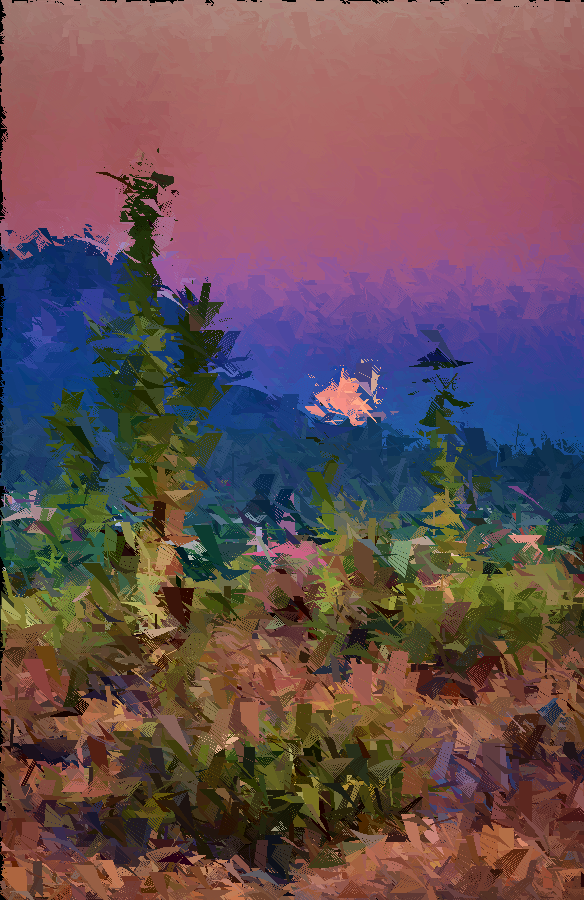
\includegraphics[width=0.4\linewidth]{final.png}
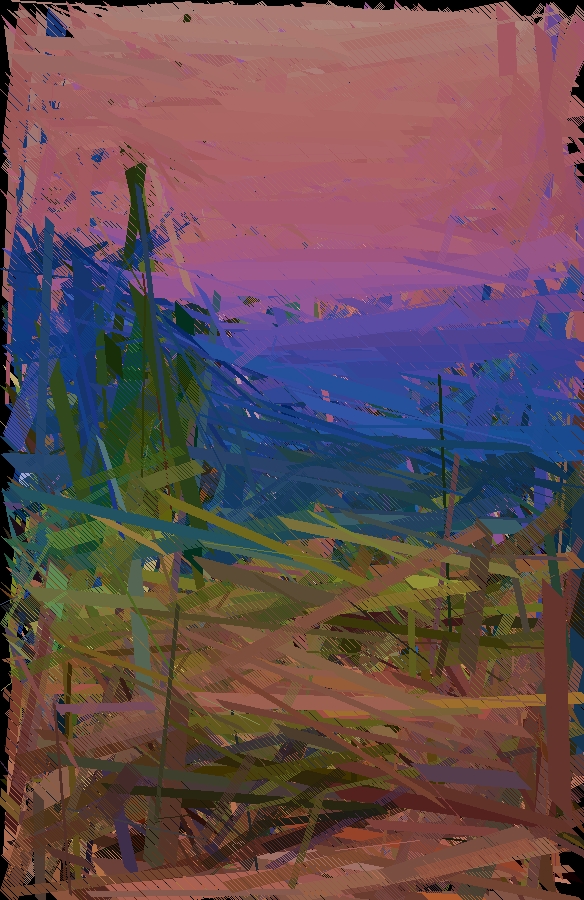
\includegraphics[width=0.4\linewidth]{informed.png}
\end{center}

More paintings can be seen in the appendix as Figure \ref{paintings}.

\subsubsection{Stroke Properties}
These two paintings ran for the same number of iterations. They show the increase in ``difficulty'' of arranging longer strokes versus shorter strokes. Through many tests, it has become apparent that a feature in a painting only shows up if the stroke length is less than that feature itself. The longer strokes tend to obscure the smaller details, like the moon in the background and some shrubbery in the foreground. In a much shorter time, a shorter-stroke painting is able to achieve a much higher fitness than another painting of longer strokes. So, one way to maximize fitness is to just have shorter strokes. Thinner strokes also have this effect but it is not as dramatically as shorter strokes. This ``impressionist'' style of painting strikes a great balance of computational work to good results, requiring much less computation for much more fit results.  For the sake of exploring other styles, we then chose to move on to the more challenging longer-stroke version and see how much improvement can be made.

\subsubsection{Selectors}
When trying to maximize fitness, it is intuitive to use the maximize selector. This is the selector that selects the most fit members of the population to mate for the next generation. It does increase the run-time dramatically, as at every iteration it must find the most fit members to mate, but the increase in fitness makes this trade-off worth it. Using the maximize selector to run a genetic algorithm for some amount of time hours will result in a higher fitness than using a tournament selector for the same amount of time. Technically, the tournament selector can get through many more iterations in the same time, but each individual iteration has a lesser positive impact on the fitness. 




\subsection{Hamming Walls}
\begin{figure}[t]
\centering
    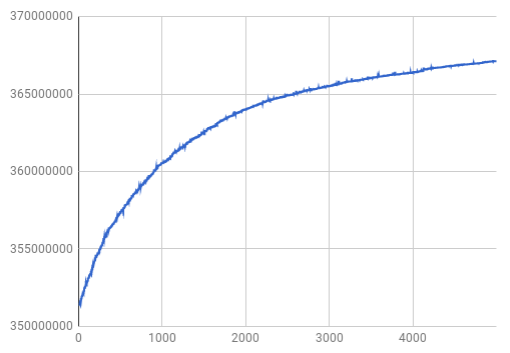
\includegraphics[width=0.6\linewidth]{2018-04-03-203542_510x353_scrot.png}
    \caption[Maximize selector fitness graph]{A graph of the maximal fitness throughout one execution of the genetic algorithm.}
    \label{fig:fitnessgraph}
\end{figure}
When looking at the fitness graph of an execution of our genetic algorithm, it takes a logarithm, or inverse-exponential, shape. This can be seen in Figure \ref{fig:fitnessgraph}. We postulate that this is due to a local maxima, or Hamming wall as they are called in genetic algorithms. This postulated maxima can be seen in Figure \ref{fig:hamming}. This is a place where an increase in fitness would require many changes to happen simultaneously.\cite{hamming} It could also be due to approaching the most optimal arrangement of strokes, but as a perfect fitness value is much higher than those values these lines are asymptotically approaching, this seems unlikely. 

More evidence for the existence of a Hamming wall can be seen in Figure \ref{fig:informedandrandom}. If the posited hamming wall was actually an optimal arrangement of strokes, then the fitness graph for the random generator execution should approach the same optimal arrangement as the informed random generator execution, around $368,000,000$, and then start to flatten out. Instead, it reaches its own Hamming wall around $351,000,000$. 
%Further evidence of hamming walls appears in the random graph - the initial slope is higher than the final slope of the random

\begin{figure}[b]
    \centering
    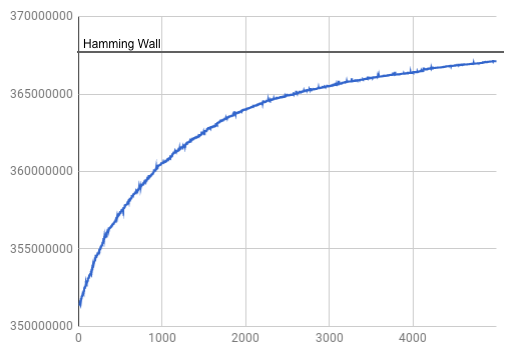
\includegraphics[width=0.6\linewidth]{hamming_graph.png}
    \caption[Visualized Hamming wall]{A fitness graph with a Hamming wall visualized. The Hamming wall is around fitness = $368,000,000$.}
    \label{fig:hamming}
\end{figure}

\begin{figure}
    \centering
    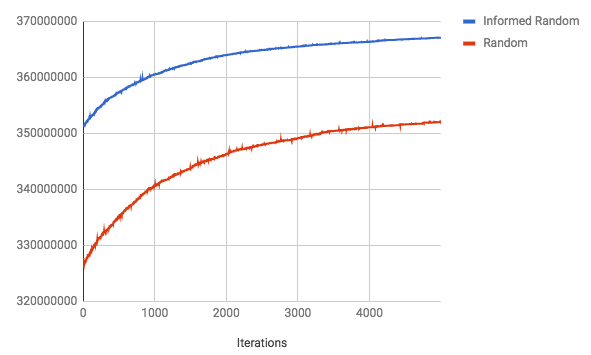
\includegraphics[width=0.6\linewidth]{InformedvsRandom.png}
    \caption[Informed random and random generator fitness graphs]{The fitness graph of two executions using an informed random and a random generator function.}
    \label{fig:informedandrandom}
\end{figure}
If one is familiar with Hamming walls, they may have heard of Gray coding. Hamming walls can be combated with something called Gray coding\cite{hamming} when using binary strings to represent members of the population. As our approach to using genetic algorithms on paintings does not use a binary-based representation, these methods of Gray coding are unfortunately not applicable. There may be ways to apply the strategies of Gray coding to our application, but they are not obvious at this point. 

Hamming walls, or local maxima in general, occur when an algorithm cannot see far enough in the future to make a change that will temporarily distance itself from its goal but eventually get it closer. When thinking about them in this sense, any part of our algorithm that greedily grabs the best option could be causing this phenomenon. The most obvious candidate is the maximize selector, which always grabs the most fit members of the population. For many iterations, that most fit member may not actually change at all, resulting in a lot of children with the same or extremely similar characteristics being added over and over again. Over a longer time, it is theoretically possible that a sudden mutation and more fit child could cause a spike and an overcoming of a Hamming wall.

Increasing the previously mentioned mutation strength would increase the probability of being able to overcome a Hamming wall. We tested raising the mutation strength until it was detrimental to the overall fitness and it never was able to overcome Hamming walls. %TODO graph

\subsubsection{Overcoming Hamming Walls with Selector Choice}

Discouraged by this Hamming wall, we turned to the tournament selector. It was touched on before, but for the sake of detail: the tournament selector works by selecting tournaments out of the total population. These tournaments each have $x$ participants, where $x$ is less than half of the population. It then picks the most fit two participants to make a child for the next iteration. This selector can sometimes be quicker than the maximize selector as you will only need to calculate the fitness of the tournament participants, not the entire genetic algorithm. This can also help avoid Hamming walls, as it will often not select the most fit or most optimal path for the next iteration. This results in a more flat, but perhaps more consistent, slope. 

Figure \ref{fig:tournament} shows the maximal fitness of every iteration using the tournament selector. Notice that it is more linear shaped, and less logarithmic, which is good when hoping to avoid asymptotically approaching a Hamming wall.
\begin{figure}
    \centering
    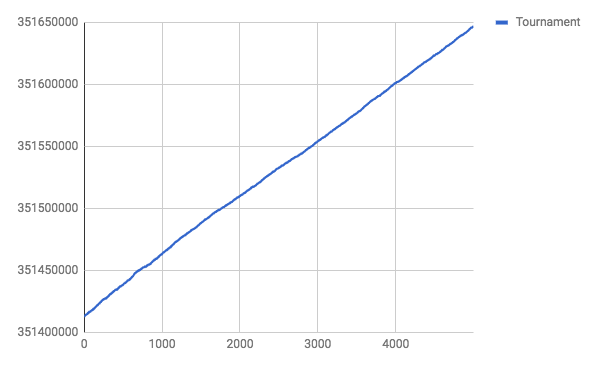
\includegraphics[width=0.6\linewidth]{Tournament.png}
    \caption[Tournament selection maximum fitness graph]{The maximum fitness of every iteration using the tournament selector. }
    \label{fig:tournament}
\end{figure}

This optimistically linear slope is immediately overshadowed when the tournament selector graph is plotted along with the maximize selector graph. This can be seen in Figure \ref{fig:tournamentvsmaximize}.
\begin{figure}
    \centering
    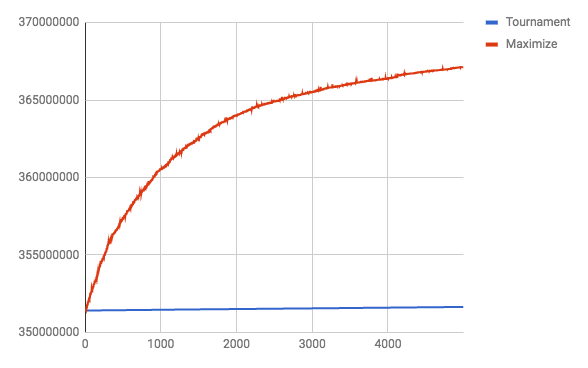
\includegraphics[width=0.65\linewidth]{TournamentvsMaximize.png}
    \caption[Tournament selector fitness graph versus maximal selector fitness graph]{The tournament selector's maximal fitness at every iteration graphed with the maximize selector's.}
    \label{fig:tournamentvsmaximize}
\end{figure}
Clearly, the maximize selector is far more effective. The postulated Hamming wall is so far above anything the tournament selector achieved in the same number of iterations. The genetic algorithm with a tournament selector would have to run for approximately $190,503$ iterations in order to overcome the one using a maximize selector's fitness. As the maximize selector took about $17$ hours to run $5000$ iterations and the tournament selector took about $13$ hours to do $5000$ iterations. The tournament selector would have to run for roughly $494$ hours, or $41$ days straight on our systems to even approach the Hamming wall of the maximize selector, assuming the linear slope would continue and it would not encounter its own Hamming wall at an earlier point. In that same time, the maximize selector would still be either slowly approaching the Hamming wall, or could be even higher than it. The amount of time required to achieve a comparable result with the tournament selector makes this approach not worth it unless running the genetic algorithm for a very long time. Lowering the tournament selector's parameters to do less tournaments or less participants in the tournaments does make it run faster but has a dramatically negative impact on the its slope. The increase in speed is not big enough to compensate for this negative impact on the slope. This can be seen in Figure \ref{fig:smallTourn}. The parameters of these two executions can be seen in Table \ref{table:tournTable}. 

\begin{figure}
    \centering
    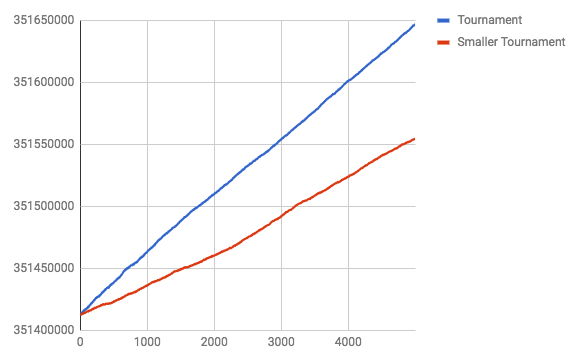
\includegraphics[width=0.6\linewidth]{SmallTournament.png}
    \caption[Tournament selector comparison]{The fitness graphs of our tournament size and a smaller tournament size.}
    \label{fig:smallTourn}
\end{figure}

\begin{table}[]
\centering
\caption{Parameters of the tournament selector executions}
\label{table:tournTable}
\begin{tabular}{lllll}
                   & Number of Tournaments & Tournament Size & Runtime  & Final Fitness \\
Tournament         & $\frac{n}{6}$         & $\frac{n}{10}$      & 13:12:52      & 351646879     \\
Smaller Tournament & $\frac{n}{10}$        & $\frac{n}{12}$      & 11:47:50      & 351554728    
\end{tabular}
\end{table}

From this test and similar ones, we deduced that it is not worth it to pursue smaller tournament parameters for more quick execution. The better balance of computational work and fitness is therefore in the larger tournament selector, but the best balance is still found in the maximize selector.

Due to these above factors, we moved on from tournament selection and used maximize selection for all tests after that.

\subsection{The Impact of Population Size}
\begin{figure}
    \centering
    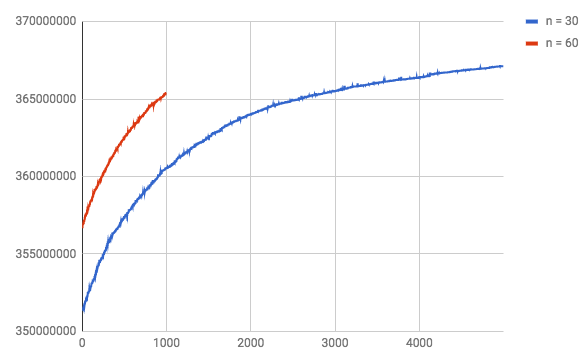
\includegraphics[width=0.7\linewidth]{popsize.png}
    \caption[Fitness graph of different population levels]{The fitness graph of two executions of the genetic algorithm: one with the population set to $n = 30$ and one with the population set to $n = 60$.}
    \label{fig:popsize}
\end{figure}
The size of the population in each iteration turns out to have a significant impact on the shape of the fitness graph. Unfortunately, it also increases the time it takes to execute one iteration greatly. 

For all executions mentioned up until this point, the population value has been set to $n = 30$. Figure \ref{fig:popsize} shows what happens when we increased the population size to $n = 60$, using our maximize selector. Unfortunately, it took so long to run, we were only able to run it out to a thousand iterations. But clearly the impact is massive. The slope at every point is higher and the initial fitness is higher. This makes sense from a conceptual perspective, with more population being generated in the beginning, there are more combinations of strokes and therefore a higher likelihood of more fit paintings being generated. Unfortunately, to run these $1000$ iterations took $69.18$ hours. Recall that running $5000$ iterations with $n = 30$ took only around $17$ hours. We found that doubling the population size  increases the amount of time required to run one iteration by a factor of $20.347$, on average. This means that increasing the population size is not as efficient as running a lower population for a longer time.

Some more examples of paintings and their reference images can be seen in the appendix as Figures \ref{fig:dadpics}, \ref{fig:guitarpics}, \ref{fig:hotairpics},  and \ref{fig:houstonpics}.


\subsection{The Impact of Iterations}
\begin{figure}
    \centering
    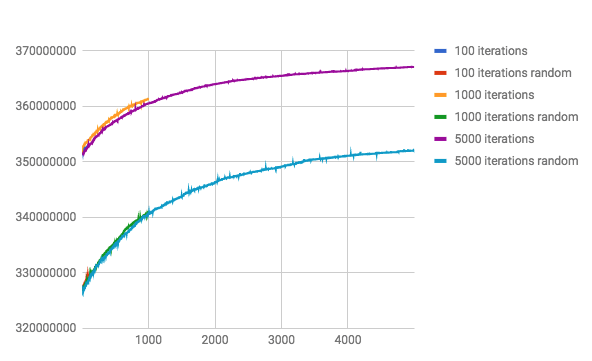
\includegraphics[width=0.8\linewidth]{randomIter.png}
    \caption[Fitness graph of multiple executions with varying amounts of iterations]{The fitness graphs of six executions, three of which used a random generator function and three didn't, of varying lengths (amounts of iterations).}
    \label{fig:iterationtests}
\end{figure}

The amount of iterations an execution has exerts a very predictable effect on the fitness graph. Shown in Figure \ref{fig:iterationtests}, the number of iterations merely determines how far along this logarithmic curve it goes. Note that even when a random generator is used, giving a lower fitness to start with, the pattern persists. 



\section{Future Work}
In the future, we hope to look into how to implement Gray coding for a project like this to avoid Hamming walls. New methods of combating Hamming walls may be needed in order to solve the problem in this context. We also hope to test more parameter configurations for our selectors, finding more optimal configurations. Lastly, we feel that implementing a more intelligent fitness function, maybe something that uses edge detection or something along those lines, could result in a more accurate evolution.
% Implementing Gray Coding
% Optimizing the selector/using tournament 
% More rigorous fitness function


\section{Introduction}
These are instructions for authors typesetting for the {\em CSCE} 
(Monte Carlo Resort, Las Vegas, Nevada, U.S.A.). This 
template has been prepared using the required format (Microsoft Word version 6.0 or later). 

\subsection{Instructions for authors}
An electronic copy of your {\em full camera-ready paper} must be uploaded (in PDF format) 
to Publication Web site before the announced deadline. Please follow the submission 
instructions shown on the web site. The URL to the website is included in the 
notification of acceptance that has been emailed to you by Prof. Arabnia.

\section{Formatting Instructions}
Please use the styles contained in this document for: Title, Abstract, Keywords, 
Heading 1, Heading 2, Body Text, Equations, References, Figures, and Captions. 
Do not add any page numbers and do not use footers and headers (it is ok to have footnotes).

\subsection{Length}
The maximum allowed number of pages is seven for Regular Research Papers (RRP) 
and Regular Research Reports (RRR); four for Short Research Papers (SRP); and two for Posters (PST).

\subsection{Title}
Type the title approximately 2.5 centimeters (1 inch) below the first line of the 
page and use 20 points type-font size in bold. Center the title (horizontally) on the page. 
Leave approximately 1 centimeter (0.4- inches) between the title and the name and 
address of yourself (and of your co-authors, if any.) Type name(s) and address(s) in 11 points 
and center them (horizontally) on the page. Note that authors are advised not to include 
their email addresses (unless they really want to.)

\subsection{Section Headings and Subsection Headings}
Number section and subsection headings consecutively in numbers and type 
them in bold. Use point size 14 for section headings and 12 for subsection headings. 
Avoid using too many capital letters. Both section headings and 
subsection headings should be flushed left.

\subsection{Main Text}
Use at least 2 centimeters (0.75 inch) for the left and right margins. 
Leave a 0.6 centimeters (0.25 inch) space between the two columns in the 
center of the page. Use font size (character size) 10 for text. The text 
should be prepared with single line spacing. Do not use bold in the main text. 
{\em If you want to emphasize specific parts of the main text, use italics.} Leave a 
2.5 centimeters (1.0 inch) margin at the page head (top of each page) for placing 
final page numbers and headers (final page numbers and running heads will be inserted 
by the publisher). Select a standard size paper such as A4 (210 X 297 mm) or letter 
(8.5 X 11 in) when preparing your manuscript.


\subsection{Tables}\label{sec:table}
All tables must be numbered consecutively. Table headings should be placed 
above the table. Tables should be as close as possible to where they 
are mentioned in the main text. Tables can span the two columns if 
need be within the page margins.

If you wish to produce publication quality tables, using the \texttt{booktabs} package is recommended.
It inserts an appropriate vertical spacing between horizontal rules and the texts, and allows you to easily handle the line thickness (the default setting is good enough though).
Table~\ref{tab:table_example} is an example from the documentation of the \texttt{booktabs} package \cite{booktabs_doc}.

\begin{table}[htb]\centering
\caption{An example of table.}\label{tab:table_example}
\begin{tabular}{@{}llr@{}} \toprule
\multicolumn{2}{c}{Item} \\ \cmidrule(r){1-2}
Animal & Description & Price (\$)\\ \midrule
Gnat & per gram & 13.65 \\
      & each      & 0.01 \\
Gnu   & stuffed   & 92.50 \\
Emu   & stuffed   & 33.33 \\
Armadillo & frozen & 8.99 \\ \bottomrule
\end{tabular}
\end{table} 


\subsection{Figures}\label{sec:figure}
All illustrations, drawings, and photographic images will be printed in black 
and white. We recommend that you examine a printed copy of your paper (in black 
and white) and make the final adjustments before submission. All illustrations 
must be numbered consecutively (i.e., not section-wise). Center the figure captions 
beneath the figure. Do not assemble figures at the back of your article, but 
place them as close as possible to where they are mentioned in the main text. 


In \LaTeX, we typically insert a figure in a floating environment using a graphic package, such as \texttt{graphicx}, \texttt{epsfig}, or \texttt{pgf}.
To specify the size of the figure, it is better to give a relative value than an absolute one.
For example,  \verb|\includegraphics[|\textit{Option}\verb|]{drawing}|, where \textit{Option} is \verb|width=\columnwidth|, assures that the width of the figure matches the width of the column.
You can specify a fraction of the value, such as \verb|.8\columnwidth|, which means to specify 80~\% of the column width.
When you refer a figure number, first make sure \verb|\label| command immediately comes after \verb|\caption| command in order for \LaTeX\ to correctly memorize the figure number. 
%%In this sample, typing \verb|Figure~\ref{fig:drawing_sample}| then yields Figure~\ref{fig:drawing_sample}.

%%\begin{figure}[htp]\centering
%%\includegraphics[width=.8\columnwidth]{drawing}
%%\caption{A sample of drawing.}\label{fig:drawing_sample}
%%\end{figure}

Figures can span the two columns if need be within the page margins.
Using the \texttt{figure*} environment will do the job in \LaTeX\ (similarly the \texttt{table*} environment for wide tables) ; however, those environments only place the floats at the top of the page, and option \texttt{[b]} and \texttt{[h]} are ignored.
In order to prevent the figures from being placed out-of-order when using both normal and starred floating environments, 
the \texttt{fixltx2e} package should be used.
%%An example of wide figure is shown in Figure~\ref{fig:wide_figure}.

%%\begin{figure*}\centering
%%  \epsfig{file=sample_wide,width=.9\textwidth}
%%\caption{Example of a wide figure.}\label{fig:wide_figure}
%%\end{figure*}

For more details, consulting resources is recommended.  You should check the book from Lamport \cite{Lamport}, and numerous online resources are also available; for example, many useful tips can be found in the \LaTeX\ Wikibooks \cite{LaTeXWikibook}.

\subsection{Mathematical formulas}\label{sec:math}
Mathematical formulas should be roughly centered and numbered, as in: 
\begin{equation}
  y = f(x)
\end{equation}

American Mathematical Society (AMS) provides a lot of useful math environments. Here are some sample equations from  the documentation of the \texttt{amsmath} package \cite{amsmathdoc} with some modifications.

A sample of using the \texttt{split} environment:
\begin{equation}\label{eqn:split}
\begin{split}
a& =b+c-d\\
 & \quad +e-f\\
 & =g+h\\
 & =i
\end{split}
\end{equation}

A sample of using the \texttt{multiline} environment:
\begin{multline}
y = a+b+c+d+e+f+g+h+i+j+k\\
+l+m+n+o+p+q+r
\end{multline}

A sample of using the \texttt{gather} environment:
\begin{gather}
a_1=b_1+c_1\\
a_2=b_2+c_2-d_2+e_2
\end{gather}

A sample of using the \texttt{align} environment with each line numbered:
\begin{align}
a_1& =b_1+c_1\\
a_2& =b_2+c_2-d_2+e_2
\end{align}
Using the same environment but only the last line is numbered:
\begin{align}
a_1& =b_1+c_1 \nonumber\\
   & =b_2+c_2-d_2+e_2
\end{align}


A sample of treating multiple lines as a block by using the \texttt{aligned} environment:
\begin{equation}
\left.\begin{aligned}
  B’&=-\partial\times E,\\
  E’&=\partial\times B - 4\pi j,
\end{aligned}
\right\}
\qquad \text{Maxwell's equations}
\end{equation}

A sample of using the \texttt{cases} environment:
\begin{equation}
P_{r-j}=\begin{cases}
    0& \text{if $r-j$ is odd},\\
    r!\,(-1)^{(r-j)/2}& \text{if $r-j$ is even}.
  \end{cases}
\end{equation}




\subsection{References}
Number in square brackets (``[ ]'' as in Secion~\ref{sec:table}, \ref{sec:figure}, and \ref{sec:math}) should cite references to 
the literature in the main text. List the cited references in numerical order at 
the very end of your paper (under the heading `References'). Start each 
referenced paper on a new line (by its number in square brackets).

Examples of reference items of different categories shown in the
References section include:

\begin{itemize}
\item example of a book in \cite{IEEEexample:book}
\item example of a book in a series in \cite{IEEEexample:bookwithseriesvolume}
\item example of a journal article in \cite{IEEEexample:article_typical}
\item example of a conference paper in \cite{IEEEexample:confwithpaper}
\item example of a patent in \cite{IEEEexample:uspat}
\item example of a website in \cite{IEEEexample:IEEEwebsite}
\item example of a web page in \cite{IEEEexample:shellCTANpage}
\item example of a databook as a manual in \cite{IEEEexample:motmanual}
\item example of a datasheet in \cite{IEEEexample:datasheet}
\item example of a master's thesis in \cite{IEEEexample:masterstype}
\item example of a technical report in \cite{IEEEexample:techreptype}
\item example of a standard in \cite{IEEEexample:standard}
\end{itemize}

\subsection{Page numbering}
{\em Do not number any pages in your paper and do not reference page numbers in the text.}

\subsection{Fine Tuning}
Do not end a page with a section or subsection heading. Keep footnotes to a minimum. 
Proper usage of the English language is expected of all Camera-Ready papers.

\subsection{Finalization}
After proofreading the final draft of the manuscript, convert it to PDF.  (Use of 
Adobe Acrobat PDF converter is strongly recommended). Examine all pages of the 
final PDF version before submission. {\em Be sure not to include a cover page, and do 
not password protect the pdf file (no security encryption). Also do not include any blank pages}

\section{Conclusions}\label{sec:conclusion}
This sample paper presents the formatting instructions for camera-ready paper 
submissions to CSCE.  Please address any problems related to use of this 
template to Kaveh Arbtan by Email (\texttt{Kaveh@ucmss.com}).

%%%%%%%%%%%%%%%%%%%%%%%%%%%%%%%%%%%%%%%%%%%%%%%%%%%%%%%%%%%%
%%
%% Reference
%% Below is an example of bibliography that contains all entries within this document.
%% You can also let BibTeX generate your bibliography by inserting the following two commands:
%%
%% \bibliographystyle{IEEEtran}
%% \bibliography{<your_bibliography_file_1>,<your_bibliography_file_2>,...}
%%
%% Note that you need to make sure that LaTeX (BibTeX) can find IEEEtrans.bst in your system.
%% If you are unsure about that, just place IEEEtrans.bst in the same directory where your LaTeX source files reside.
%%
%%%%%%%%%%%%%%%%%%%%%%%%%%%%%%%%%%%%%%%%%%%%%%%%%%%%%%%%%%%%%
%%% Below thebibliography environment will be automatically created in a different file (your_file_name.bbl) 
%%% if you use BibTeX and specify IEEEtrans.bst.


\begin{thebibliography}{1}
\providecommand{\url}[1]{#1}
\csname url@rmstyle\endcsname
\providecommand{\newblock}{\relax}
\providecommand{\bibinfo}[2]{#2}
\providecommand\BIBentrySTDinterwordspacing{\spaceskip=0pt\relax}
\providecommand\BIBentryALTinterwordstretchfactor{4}
\providecommand\BIBentryALTinterwordspacing{\spaceskip=\fontdimen2\font plus
\BIBentryALTinterwordstretchfactor\fontdimen3\font minus
  \fontdimen4\font\relax}
\providecommand\BIBforeignlanguage[2]{{%
\expandafter\ifx\csname l@#1\endcsname\relax
\typeout{** WARNING: IEEEtran.bst: No hyphenation pattern has been}%
\typeout{** loaded for the language `#1'. Using the pattern for}%
\typeout{** the default language instead.}%
\else
\language=\csname l@#1\endcsname
\fi
#2}}

\bibitem{booktabs_doc}
\BIBentryALTinterwordspacing
Simon Fear. (2005). Publication quality tables in LaTeX. [Online]. Available:
\url{http://www.ctan.org/tex-archive/macros/latex/contrib/booktabs/booktabs.pdf}
\BIBentrySTDinterwordspacing

\bibitem{Lamport}
Leslie Lamport.
\newblock {\em ``LaTeX:  A Document Preparation System.''}
\newblock Addison-Wesley Publishing Company, 1986.

\bibitem{LaTeXWikibook}
\BIBentryALTinterwordspacing
Wikibooks contributors. (2008)  LaTeX Wikibooks, collection of open-content textbooks. [Online]. Available: \url{http://en.wikibooks.org/wiki/LaTeX}
\BIBentrySTDinterwordspacing

\bibitem{amsmathdoc}
\BIBentryALTinterwordspacing
American Mathematical Society. (1999) User's Guide for the amsmath Package (Version 2.0). [Online]. Available:
\url{ftp://ftp.ams.org/pub/tex/doc/amsmath/amsldoc.pdf}
\BIBentrySTDinterwordspacing

% \bibitem{Resrc}
% Ree Source Person.
% \newblock ``Title of Research Paper''; name of journal (name of publisher of the journal), 
% Vol. No., Issue No., Page numbers (eg.728--736), Month, and Year of publication (e.g., Oct~2006).

\bibitem{IEEEexample:book}
S.~M. Metev and V.~P. Veiko, \emph{Laser Assisted Microtechnology}, 2nd~ed.,
  R.~M. Osgood, Jr., Ed.\hskip 1em plus 0.5em minus 0.4em\relax Berlin,
  Germany: Springer-Verlag, 1998.

\bibitem{IEEEexample:bookwithseriesvolume}
J.~Breckling, Ed., \emph{The Analysis of Directional Time Series: Applications
  to Wind Speed and Direction}, ser. Lecture Notes in Statistics.\hskip 1em
  plus 0.5em minus 0.4em\relax Berlin, Germany: Springer, 1989, vol.~61.

\bibitem{IEEEexample:article_typical}
S.~Zhang, C.~Zhu, J.~K.~O. Sin, and P.~K.~T. Mok, ``A novel ultrathin elevated
  channel low-temperature poly-{Si} {TFT},'' \emph{{IEEE} Electron Device
  Lett.}, vol.~20, pp. 569--571, Nov. 1999.

\bibitem{IEEEexample:confwithpaper}
M.~Wegmuller, J.~P. von~der Weid, P.~Oberson, and N.~Gisin, ``High resolution
  fiber distributed measurements with coherent {OFDR},'' in \emph{Proc.
  {ECOC}'00}, 2000, paper 11.3.4, p. 109.

\bibitem{IEEEexample:uspat}
R.~E. Sorace, V.~S. Reinhardt, and S.~A. Vaughn, ``High-speed digital-to-{RF}
  converter,'' U.S. Patent 5\,668\,842, Sept. 16, 1997.

\bibitem{IEEEexample:IEEEwebsite}
\BIBentryALTinterwordspacing
(2002) The {IEEE} website. [Online]. Available: \url{http://www.ieee.org/}
\BIBentrySTDinterwordspacing

\bibitem{IEEEexample:shellCTANpage}
\BIBentryALTinterwordspacing
M.~Shell. (2002) {IEEE}tran homepage on {CTAN}. [Online]. Available:
  \url{http://www.ctan.org/tex-archive/macros/latex/contrib/supported/IEEEtran%
/}
\BIBentrySTDinterwordspacing

\bibitem{IEEEexample:motmanual}
\emph{{FLEXChip} Signal Processor ({MC68175/D})}, Motorola, 1996.

\bibitem{IEEEexample:datasheet}
``{PDCA12-70} data sheet,'' Opto Speed SA, Mezzovico, Switzerland.

\bibitem{IEEEexample:masterstype}
A.~Karnik, ``Performance of {TCP} congestion control with rate feedback:
  {TCP/ABR} and rate adaptive {TCP/IP},'' M. Eng. thesis, Indian Institute of
  Science, Bangalore, India, Jan. 1999.

\bibitem{IEEEexample:techreptype}
J.~Padhye, V.~Firoiu, and D.~Towsley, ``A stochastic model of {TCP} {R}eno
  congestion avoidance and control,'' Univ. of Massachusetts, Amherst, MA,
  CMPSCI Tech. Rep. 99-02, 1999.

\bibitem{IEEEexample:standard}
\emph{Wireless {LAN} Medium Access Control {(MAC)} and Physical Layer {(PHY)}
  Specification}, IEEE Std. 802.11, 1997.

\end{thebibliography}


\end{document}
